%------------------------------------------------------------------%
% Cannabis Data Science Presentation
% Date: 11/17/2021
% Authors: Keegan Skeate <keegan@cannlytics.com>
% Copyright (c) Cannlytics
%------------------------------------------------------------------%
\documentclass[xcolor={dvipsnames}]{beamer}
\hypersetup{pdfpagemode=FullScreen}
\mode<presentation>{
  \usetheme{Boadilla}
  \usecolortheme{orchid}
  \usefonttheme{default}
  \setbeamertemplate{navigation symbols}{}
  \setbeamertemplate{caption}[numbered]
} 
\setbeamersize{text margin left=0.5in,text margin right=0.5in}

%------------------------------------------%
% Packages
%------------------------------------------%
\usepackage[english]{babel}
\usepackage[utf8x]{inputenc}
\usepackage[dvipsnames]{xcolor}
\usepackage{amsmath}
\renewcommand*\footnoterule{} % No sperating line on footnote.
\usepackage{mathtools} % Annotating equations.
\usepackage{hhline} % Provides doublebars.
\usepackage[super]{nth} % Adds easy 1st, 2nd, 3rd, etc. for numbers.
\usepackage{graphicx, caption, subcaption} % Makes putting captions on figures easy.
\usepackage{tikz} 
\usepackage{xparse}

%------------------------------------------%
% Style
%------------------------------------------%
\definecolor{DarkGreen}{RGB}{2, 48, 32}
\definecolor{CalyxGreen}{RGB}{34, 153, 84}
\definecolor{DarkOrange}{RGB}{199, 0, 57}
\definecolor{LightOrange}{RGB}{255, 87, 51}
\definecolor{LightGreen}{RGB}{218, 247, 166}
\definecolor{LightYellow}{RGB}{255, 195, 0}
\setbeamercolor*{palette primary}{bg=LightGreen, fg=DarkGreen}
\setbeamercolor*{palette secondary}{bg=LightGreen, fg=DarkGreen}
\setbeamercolor*{palette tertiary}{bg=LightGreen, fg=DarkGreen}

%------------------------------------------%
% Commands
%------------------------------------------%
% Struts.
\newcommand\T{\rule{0pt}{2.5ex}} % Top-strut.
\newcommand\B{\rule[-1.25ex]{0pt}{0pt}} % Bottom-strut.
\newenvironment<>{varblock}[2][.9\textwidth] % Resized blocks.
  {\setlength{\textwidth}{#1}
  \begin{actionenv}#3
    \def\insertblocktitle{#2}\par
    \usebeamertemplate{block begin}}
  {\par\usebeamertemplate{block end}
  \end{actionenv}}
 
% Large balls
\defbeamertemplate{enumerate item}{largeball}
{\begin{pgfpicture}{-1ex}{-0.65ex}{1.5ex}{1.5ex}
\usebeamercolor[fg]{item projected}
{\pgftransformscale{2.5}\pgftext{\Large\pgfuseshading{bigsphere}}}
{\pgftransformshift{\pgfpoint{0pt}{0.5pt}}
\pgftext{\usebeamerfont*{item projected}\small\insertenumlabel}}
\end{pgfpicture}}

% Fancy arrows.
\NewDocumentCommand\UpArrow{O{2.0ex} O{black}}{%
   \mathrel{\tikz[baseline] \draw [->, line width=0.5pt, #2] (0,0) -- ++(0,#1);}} % Fancy up-arrow.
\NewDocumentCommand\DownArrow{O{2.0ex} O{black}}{%
   \mathrel{\tikz[baseline] \draw [<-, line width=0.5pt, #2] (0,0) -- ++(0,#1);}} % Fancy down-arrow.

% Align equations on the left.
\makeatletter
\newcommand{\LeftEqNo}{\let\veqno\@@leqno}
\makeatother

%------------------------------------------------------------------%
% Title
%------------------------------------------------------------------%
\title[Meetup Group]{}
\author{Cannabis Data Science}
\institute[]{\Large Meetup Group}
\date{November \nth{17}, 2021}
\begin{document}
\begin{frame}{}
  
\includegraphics[scale=0.075]{images/logos/cannlytics_logo_with_text_light.png}
  \titlepage
\end{frame}

%------------------------------------------------------------------%
% Introduction
%------------------------------------------------------------------%

\section{Introduction}

\begin{frame}{}

{\large Predicting Market Performance}\vspace{\baselineskip}\\

\begin{center}
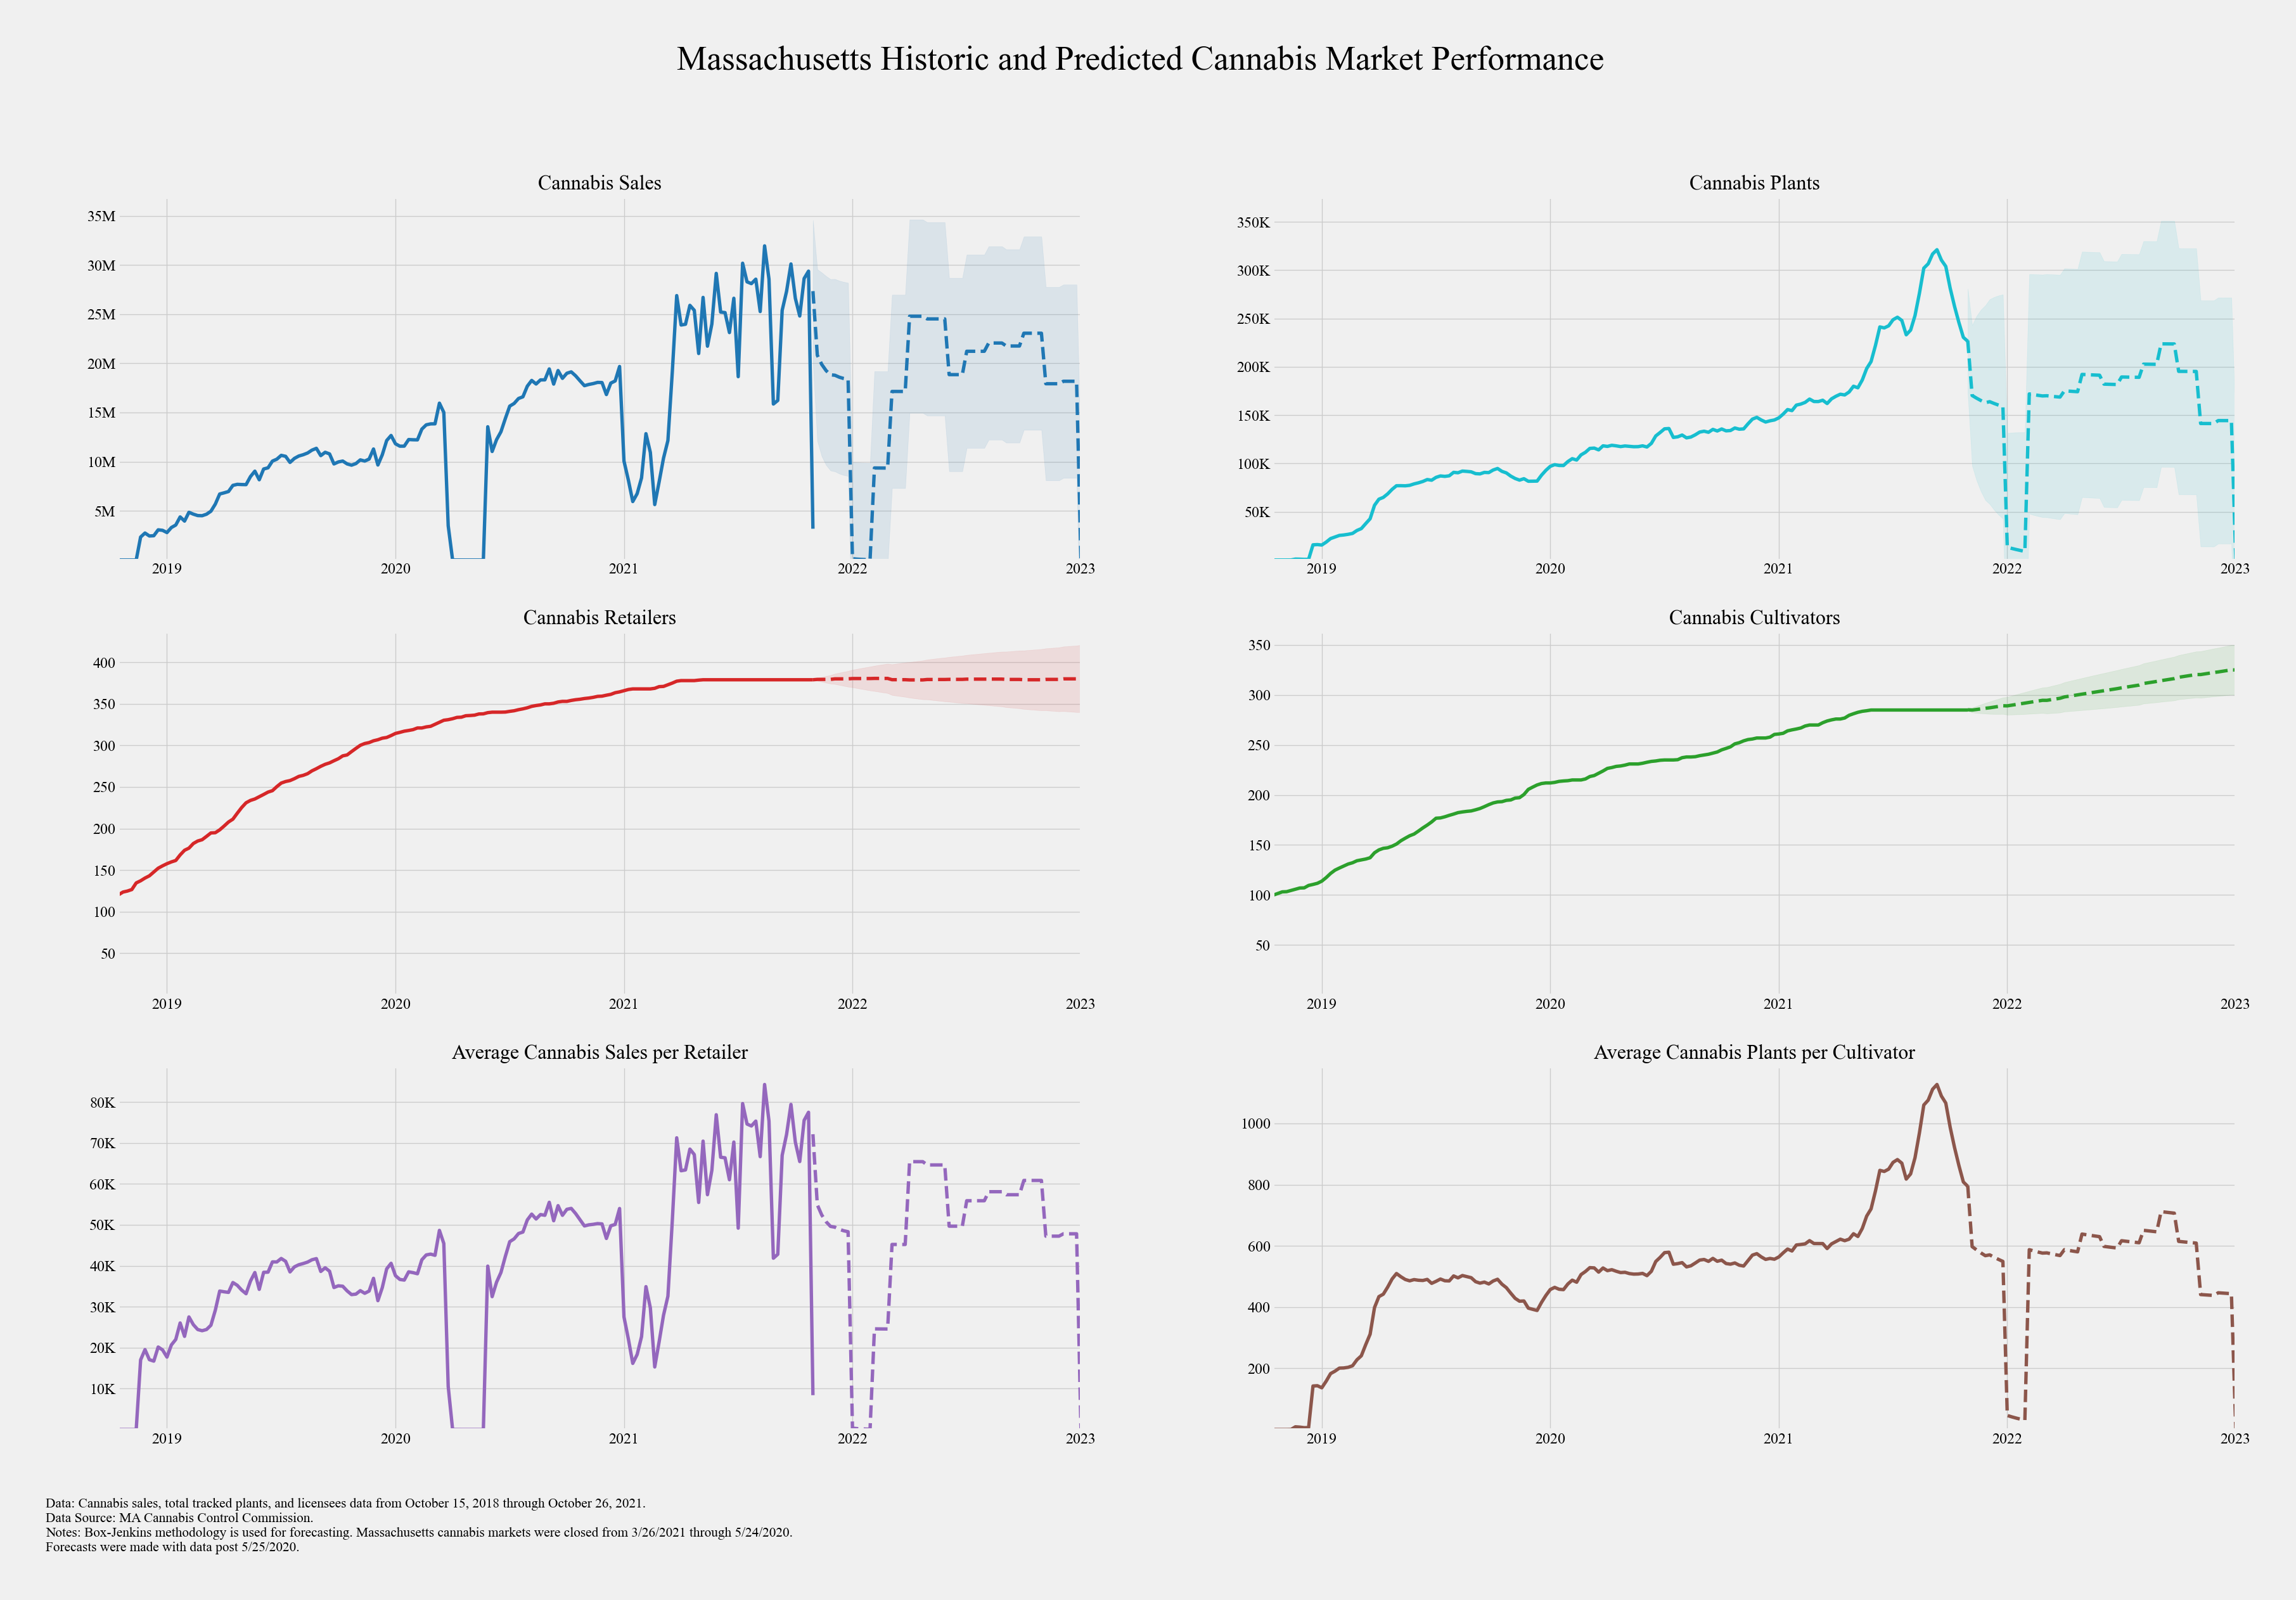
\includegraphics[width=\textwidth]{images/ma_market_forecast.png}
\end{center}

\end{frame}


\section{Theoretical Economics}

% Productivity slide.

\begin{frame}{}

{\large Productivity}

\vspace{.75\baselineskip}

\begin{itemize}
\item Output ($Y$): sales per week.
\vspace{.75\baselineskip}
\item Total factor of productivity ($A$).
\vspace{.75\baselineskip}
\item Labor hours ($L$): labor hours per week.
\vspace{.75\baselineskip}
\item Total capital ($K$): flowering plants per week.
\end{itemize}

{\large Cobb-Douglas Production Function}

\vspace{.75\baselineskip}

$$Y_t = AK_t^{\alpha}L_t^{\beta}$$

\end{frame}

% MPL and Wage

\begin{frame}{}

{\large Marginal Product of Labor and Competitive Wages}

\vspace{.75\baselineskip}

$$Y_t = AK_t^{\alpha}L_t^{\beta}$$

$$MPL_t = \beta AK_t^{\alpha}L_t^{\beta - 1}$$

$$MPL_t = \beta \frac{Y_t}{L_t}$$

$$w_t^* = MPL_t = \beta \frac{Y_t}{L_t}$$


\end{frame}

% MPK and Interest Rate

\begin{frame}{}

{\large Marginal Product of Capital and Competitive Interest Rate}

\vspace{.75\baselineskip}

$$Y_t = AK_t^{\alpha}L_t^{\beta}$$

$$MPK_t = \alpha AK_t^{\alpha - 1}L_t^{\beta}$$

$$MPK_t = \alpha \frac{Y_t}{K_t}$$

$$r_t^* = MPK_t = \alpha \frac{Y_t}{K_t}$$


\end{frame}


\section{Empirical Economics}

% Slide on empirical estimation.

\begin{frame}{}

``The questions concerning what number of firms is too large to permit collusion, and what amount of output control is sufficient for price setting, are essentially empirical issues.''

\vspace{.75\baselineskip}

{\tiny Reevaluation of the Structure-Conduct-Performance Paradigm in Banking.\\
Douglas D. Evanoff and Diana L. Fortier}

\end{frame}


\begin{frame}{}

{\large Estimation of a Cobb-Douglas Production Function}

\vspace{.75\baselineskip}

$$lnY_t = lnA + \alpha K_t + \beta L_t + \epsilon_t $$

\end{frame}

\section{Cannabis Applications}

% Rules of forecasting slide.

%\begin{frame}{}
%
%{\Large The 10 Commandments of Forecasting}\vspace{\baselineskip}\\
%
%\begin{enumerate}
%\item Know what you are forecasting.
%\item Understand the purpose of forecasting.
%\item Acknowledge the cost of the forecast error.
%\item Rationalize the forecast horizon.
%\item Understand the choice of variables.
%\item Rationalize the forecasting model used.
%\item Know how to present the results.
%\item Know how to decipher the forecast results.
%\item Use recursive methods.
%\item Understand that forecasting models evolve over time.
%\end{enumerate}
%\end{frame}

% Closing slide.

%\begin{frame}{}
%\begin{center}
%\begin{minipage}{3.85in}
%\begin{block}{Until next time}
%Study some economics, make some forecasts, and next week we can check our forecasts.
%\end{block}
%
%\end{minipage}
%\end{center}
%%
%%{\Large References}\vspace{\baselineskip}\\
%%
%%\begin{enumerate}
%%\item Inter-Industry Studies of Structure and Performance by Richard Schmalensee. Working Paper #1874-87. April 1987.
%%\end{enumerate}
%
%\end{frame}

%------------------------------------------------------------------%
\end{document}
%------------------------------------------------------------------%
